%%
%% This is file `sample-sigplan.tex',
%% generated with the docstrip utility.
%%
%% The original source files were:
%%
%% samples.dtx  (with options: `sigplan')
%% 
%% IMPORTANT NOTICE:
%% 
%% For the copyright see the source file.
%% 
%% Any modified versions of this file must be renamed
%% with new filenames distinct from sample-sigplan.tex.
%% 
%% For distribution of the original source see the terms
%% for copying and modification in the file samples.dtx.
%% 
%% This generated file may be distributed as long as the
%% original source files, as listed above, are part of the
%% same distribution. (The sources need not necessarily be
%% in the same archive or directory.)
%%
%% Commands for TeXCount
%TC:macro \cite [option:text,text]
%TC:macro \citep [option:text,text]
%TC:macro \citet [option:text,text]
%TC:envir table 0 1
%TC:envir table* 0 1
%TC:envir tabular [ignore] word
%TC:envir displaymath 0 word
%TC:envir math 0 word
%TC:envir comment 0 0
%%
%%
%% The first command in your LaTeX source must be the \documentclass command.
%\documentclass[sigplan,screen]{acmart}
\documentclass[acmsmall,screen,review,anonymous,nonacm]{acmart}
%% NOTE that a single column version is required for 
%% submission and peer review. This can be done by changing
%% the \doucmentclass[...]{acmart} in this template to 
%% \documentclass[manuscript,screen,review]{acmart}
%% 
%% To ensure 100% compatibility, please check the white list of
%% approved LaTeX packages to be used with the Master Article Template at
%% https://www.acm.org/publications/taps/whitelist-of-latex-packages 
%% before creating your document. The white list page provides 
%% information on how to submit additional LaTeX packages for 

\usepackage{mylhs2tex}
\usepackage[backend=pgf, extension=pgf, outputdir=diagrams, input]{diagrams-latex}
\usepackage{tikz}
\usepackage{tikz-cd} % for commutative diagrams
\usepackage{textgreek} % for \textlambda
\usepackage{multirow} % for multirow in tables
\usepackage[inline]{enumitem} % for inline lists
\usepackage{minted} % for code snippets
\usepackage{wrapfig} % for wrapping text around figures
\usepackage{mathpartir} % for inference rules



\newcommand{\REM}[2]{\textcolor{blue}{[\textbf{#1:} #2]}}
\newcommand{\Johan}[1]{\REM{Johan}{#1}}
\newcommand{\Matthias}[1]{\REM{Matthias}{#1}}
\newcommand{\Igor}[1]{\REM{Igor}{#1}}
\newcommand{\nm}{notional machine}
\newcommand{\nms}{notional machines}
\newcommand{\Nm}{Notional machine}
\newcommand{\Nms}{Notional machines}
\newcommand{\NM}{Notional Machine}
\newcommand{\NMs}{Notional Machines}
\newcommand{\nmName}[1]{\textsc{#1}}
\newcommand{\plName}[1]{\textsc{#1}}
\newcommand{\done}{\textcolor[rgb]{0,1,0}{(done)}}
\newcommand{\todo}{\textcolor[rgb]{1,0,0}{TODO }}
\newcommand{\inv}[1]{{#1}^{\scriptscriptstyle -1}}
\newcommand{\numOfNMs}{37\ }

\newcommand{\app}[2]{#1\ #2}
\newcommand{\abs}[2]{\text{\textlambda}#1.#2}
\newcommand{\tyabs}[3]{\text{\textlambda}#1:#2.#3}
\newcommand{\subst}[3]{[#2 \mapsto #1]#3}

\newcommand{\ift}[3]{\texttt{if\;}#1\texttt{\;then\;}#2\texttt{\;else\;}#3}
\newcommand{\succt}[1]{\texttt{succ\;}#1}
\newcommand{\predt}[1]{\texttt{pred\;}#1}
\newcommand{\iszerot}[1]{\texttt{iszero\;}#1}
\newcommand{\true}{\texttt{true}}
\newcommand{\false}{\texttt{false}}
\newcommand{\zero}{0}

\newcommand{\unit}{\texttt{unit}}
\newcommand{\refr}[1]{\texttt{ref\;}#1}
\newcommand{\deref}[1]{\texttt{!}#1}
\newcommand{\assign}[2]{#1\;:= #2}
\newcommand{\seq}[2]{#1;\;#2}
\newcommand{\proj}[2]{#1.#2}

\newcommand{\Bool}{\texttt{Bool}}
\newcommand{\Nat}{\texttt{Nat}}
\newcommand{\Ref}[1]{\texttt{Ref\;}#1}
\newcommand{\Unit}{\texttt{Unit}}
\newcommand{\Fun}[2]{#1 \rightarrow #2}
\newcommand{\Tuple}[1]{\{#1\}}

%% review and adoption.
%% Fonts used in the template cannot be substituted; margin 
%% adjustments are not allowed.
%%
%% \BibTeX command to typeset BibTeX logo in the docs
\AtBeginDocument{%
  \providecommand\BibTeX{{%
    \normalfont B\kern-0.5em{\scshape i\kern-0.25em b}\kern-0.8em\TeX}}}

%% Rights management information.  This information is sent to you
%% when you complete the rights form.  These commands have SAMPLE
%% values in them; it is your responsibility as an author to replace
%% the commands and values with those provided to you when you
%% complete the rights form.
\setcopyright{acmcopyright}
\copyrightyear{2018}
\acmYear{2018}
\acmDOI{XXXXXXX.XXXXXXX}

%% These commands are for a PROCEEDINGS abstract or paper.
\acmConference[Conference acronym 'XX]{Make sure to enter the correct
  conference title from your rights confirmation emai}{June 03--05,
  2018}{Woodstock, NY}
%
%  Uncomment \acmBooktitle if th title of the proceedings is different
%  from ``Proceedings of ...''!
%
%\acmBooktitle{Woodstock '18: ACM Symposium on Neural Gaze Detection,
%  June 03--05, 2018, Woodstock, NY} 
\acmPrice{15.00}
\acmISBN{978-1-4503-XXXX-X/18/06}


%%
%% Submission ID.
%% Use this when submitting an article to a sponsored event. You'll
%% receive a unique submission ID from the organizers
%% of the event, and this ID should be used as the parameter to this command.
%%\acmSubmissionID{123-A56-BU3}

%%
%% For managing citations, it is recommended to use bibliography
%% files in BibTeX format.
%%
%% You can then either use BibTeX with the ACM-Reference-Format style,
%% or BibLaTeX with the acmnumeric or acmauthoryear sytles, that include
%% support for advanced citation of software artefact from the
%% biblatex-software package, also separately available on CTAN.
%%
%% Look at the sample-*-biblatex.tex files for templates showcasing
%% the biblatex styles.
%%

%%
%% The majority of ACM publications use numbered citations and
%% references.  The command \citestyle{authoryear} switches to the
%% "author year" style.
%%
%% If you are preparing content for an event
%% sponsored by ACM SIGGRAPH, you must use the "author year" style of
%% citations and references.
%% Uncommenting
%% the next command will enable that style.
\citestyle{acmauthoryear}

%%
%% end of the preamble, start of the body of the document source.
\begin{document}

%%
%% The "title" command has an optional parameter,
%% allowing the author to define a "short title" to be used in page headers.
\title{Sound Notional Machines}

%%
%% The "author" command and its associated commands are used to define
%% the authors and their affiliations.
%% Of note is the shared affiliation of the first two authors, and the
%% "authornote" and "authornotemark" commands
%% used to denote shared contribution to the research.
\author{Igor Moreno Santos}
\email{igor.moreno.santos@usi.ch}
\orcid{0000-0002-7844-2058}
\affiliation{%
  \institution{Universit\`a della Svizzera italiana}
  \city{Lugano}
  \country{Switzerland}
}

\author{Matthias Hauswirth}
\email{Matthias.Hauswirth@usi.ch}
\orcid{0000-0001-5527-5931}
\affiliation{%
  \institution{Universit\`a della Svizzera italiana}
  \city{Lugano}
  \country{Switzerland}
}

\author{Johan Jeuring}
\email{j.t.jeuring@uu.nl}
\orcid{0000-0001-5645-7681}
\affiliation{%
  \institution{Utrecht University}
  \city{Utrecht}
  \country{The Netherlands}
}



%%
%% By default, the full list of authors will be used in the page
%% headers. Often, this list is too long, and will overlap
%% other information printed in the page headers. This command allows
%% the author to define a more concise list
%% of authors' names for this purpose.
%\renewcommand{\shortauthors}{Trovato and Tobin, et al.}

%%
%% The abstract is a short summary of the work to be presented in the
%% article.
\begin{abstract}
%What is a notional machine?
A notional machine is
a pedagogical device
that abstracts away details of the semantics of a programming language 
to focus on some aspects of interest.
%What properties should an NM satisfy?
A \nm{} should be \emph{sound}:
it should be consistent with the corresponding programming language,
and it should be a proper abstraction.
This reduces the risk of it introducing misconceptions in education.
% - Problem
Despite being widely used in computer science education,
\nms{}
are usually not evaluated with respect to their soundness.
% - Solution
To address this problem,
we first introduce a formal definition of soundness for \nms{}.
% -- Explain a bit the formalism
The definition is based on the construction of a commutative diagram that relates
the \nm{} with the aspect of the programming language under its focus.
%
Derived from this formalism,
we present a methodology for
%designing
constructing
sound \nms{},
which we demonstrate by
applying it to
a series of small case studies.
%
We also show how the same formalism can be used to
%Finally, we present a similar methodology to
analyze existing \nms{} and
find
inconsistences
in them
as well as
propose solutions to these inconsistencies.
%
% - Takeaways
%Our work provides a formal foundation for \nms{} and
The work establishes a firmer ground for research in notional machines
by
serving as a framework to reason about them.
%
% The result is more generally a framework to reason about notional machines
% and as such
% can be used
% in the design, analysis, and evaluation of notional machines,
% as well as
% the construction of automated tools
% based on
% %for
% notional machines.
\end{abstract}

%%
%% The code below is generated by the tool at http://dl.acm.org/ccs.cfm.
%% Please copy and paste the code instead of the example below.
%%
\begin{CCSXML}
<ccs2012>
<concept>
<concept_id>10003456.10003457.10003527</concept_id>
<concept_desc>Social and professional topics~Computing education</concept_desc>
<concept_significance>500</concept_significance>
</concept>
<concept>
<concept_id>10011007.10011006.10011039</concept_id>
<concept_desc>Software and its engineering~Formal language definitions</concept_desc>
<concept_significance>500</concept_significance>
</concept>
<concept>
<concept_id>10011007.10011006.10011050</concept_id>
<concept_desc>Software and its engineering~Context specific languages</concept_desc>
<concept_significance>500</concept_significance>
</concept>
</ccs2012>
\end{CCSXML}

\ccsdesc[500]{Social and professional topics~Computing education}
\ccsdesc[500]{Software and its engineering~Formal language definitions}
\ccsdesc[500]{Software and its engineering~Context specific languages}


%%
%% Keywords. The author(s) should pick words that accurately describe
%% the work being presented. Separate the keywords with commas.
\keywords{notional machines, programming education}

%% A "teaser" image appears between the author and affiliation
%% information and the body of the document, and typically spans the
%% page.
%\begin{teaserfigure}
%  \includegraphics[width=\textwidth]{sampleteaser}
%  \caption{Seattle Mariners at Spring Training, 2010.}
%  \Description{Enjoying the baseball game from the third-base
%  seats. Ichiro Suzuki preparing to bat.}
%  \label{fig:teaser}
%\end{teaserfigure}

%\received{20 February 2007}
%\received[revised]{12 March 2009}
%\received[accepted]{5 June 2009}

%%
%% This command processes the author and affiliation and title
%% information and builds the first part of the formatted document.
\maketitle

\section{Introduction}

\begin{wrapfigure}{r}{.50\textwidth}
%(λx.λy. x) a b
%\begin{figure}
    \centering
    \begin{diagram}[width=0.45\textwidth]
import Diagrams.Prelude hiding (trace, _fontSize)

import NotionalMachines.Lang.UntypedLambda.Main (Exp (..), parse)
import NotionalMachines.LangInMachine.UntypedLambdaExpressionTree (diagramTrace)
import NotionalMachines.Machine.ExpressionTree.BubbleDiagram (toDiagram', _fontSize, _framePadding)
import NotionalMachines.Meta.Steppable (Steppable (trace))
import NotionalMachines.Util.Diagrams (diagramWithError)
import NotionalMachines.Examples.Diagrams (langAndNMTrace)

toDia = toDiagram' (def { _fontSize = 0.12, _framePadding = 0.04 })
t = langAndNMTrace 0.05
                   (diagramTrace toDia)
                   (fmap trace . parse)

dia = (diagramWithError . t)
      "(\\t. \\f. t) a b"
    \end{diagram}
    \caption{Evaluation of the term $\texttt{\app{\app{(\abs{t}{(\abs{f}{t})})}{a}}{b}}$ shown with the \nm{} \nmName{ExpTree}.}
    \label{fig:takeFirst}
%\end{figure}
\end{wrapfigure}

% - learning programming an notional machines
Learning to program involves learning how to express a program in a programming language, 
but also learning what the semantics of such a program is. 
For novices, the semantics of a program is often not obviously apparent from the program itself.
% - what is an NM?
Instructors then often use a \emph{\nm{}}~\citep{fincherNotionalMachinesComputing2020} to help teach
some particular aspect of programs and programming languages,
and also to assess students' understanding of said aspect.
%
This aspect is the \nm{}'s focus.
%
% - an example
For example, showing expressions as trees (the \nmName{ExpTree} \nm{}),
as depicted in Figure~\ref{fig:takeFirst},
brings out the internal structure of lambda-calculus expressions~\citep{marceauValuesGrowTrees2011}
and can help to explain the step-by-step evaluation of such expressions. 
%
% Note the two dimensions that play a role here:
% showing some aspect of a programming language (showing the expression as a tree), and
% performing an operation on it (a step in the evaluation of an expression). 
%A NM should help a novice in understanding the aspects for which the NM has been designed.
\Nms{} are used widely in computer science education;
\citet{fincherNotionalMachinesComputing2020} interviewed computer science teachers
to build up a collection of over 50 \nms{}\footnote{\url{https://notionalmachines.github.io/notional-machines.html}}.


% - the quality of an NM is important.
\subsection{Unsound \NMs{}}

Given the extensive use of \nms{},
and
their intended use as devices to help students when learning,
it is important to look at their quality.
%Obviously, a \nm{} should be tested in practice
%%
%to answer questions such as
%``how well do students understand a particular aspect after studying it using a particular \nm{}?''
%and
%``what is the cost associated with introducing the notional machine
%(how much time had to be invested to obtain a benefit)?''.
%%
% But even before experimenting with a \nm{},
%%
% The first quality attribute we should be concerned with is to
To begin with,
one should
make sure that the \nm{} is \emph{sound}:
% correct
% consistent
% accurate
it is
%in some sense
faithful to the aspect of programs it is meant to focus on.
%
% Feynman quote
Anecdotal evidence of using unsound representations in education goes back a long way.
%
In 1960, education pioneer Jerome Bruner wrote that
``the task of teaching a subject to a child at any particular age is one of representing the structure of that subject in terms of the child’s way of viewing things'', that this
``task can be thought of as one of translation'', but that ideas have to be
``represented \emph{honestly} […] in the thought forms of children''~\cite{ brunerProcessEducation1960}.
Bruner’s use of the term ``honestly'' can be seen as a call for soundness of such representations.
%
Decades later,
Richard Feynman eloquently stated~\citep{feynmanSurelyYouRe1985},
after reviewing ``seventeen feet'' of new mathematics schoolbooks for the California State Curriculum Commission:

\begin{quote}
    %... the books were so lousy.
    %They were false. They were hurried.
    [The books] would try to be rigorous, but they would use examples
    (like automobiles in the street for ``sets'')
    which were almost OK, but in which there were always some subtleties.
    The definitions weren't accurate.
    Everything was a little bit ambiguous.
    %---they weren't smart enough to understand what was meant by ``rigor.''
    %They were faking it.
    %They were teaching something they didn’t understand, and
    %which was, in fact, useless, at that time, for the child.
\end{quote}

Ambiguously specified \nms{}
and
\nms{} with imperfect analogies to programming concepts
are a problem.
Educators may mischaracterize language features and
students may end up with misconceptions~\citep{chiodiniCuratedInventoryProgramming2021} instead of profoundly understanding the language.

% saves about 20 lines of text
\begin{wrapfigure}{r}{.50\textwidth}
% \begin{figure}[h]
    \centering
    \begin{tabular}{c}
        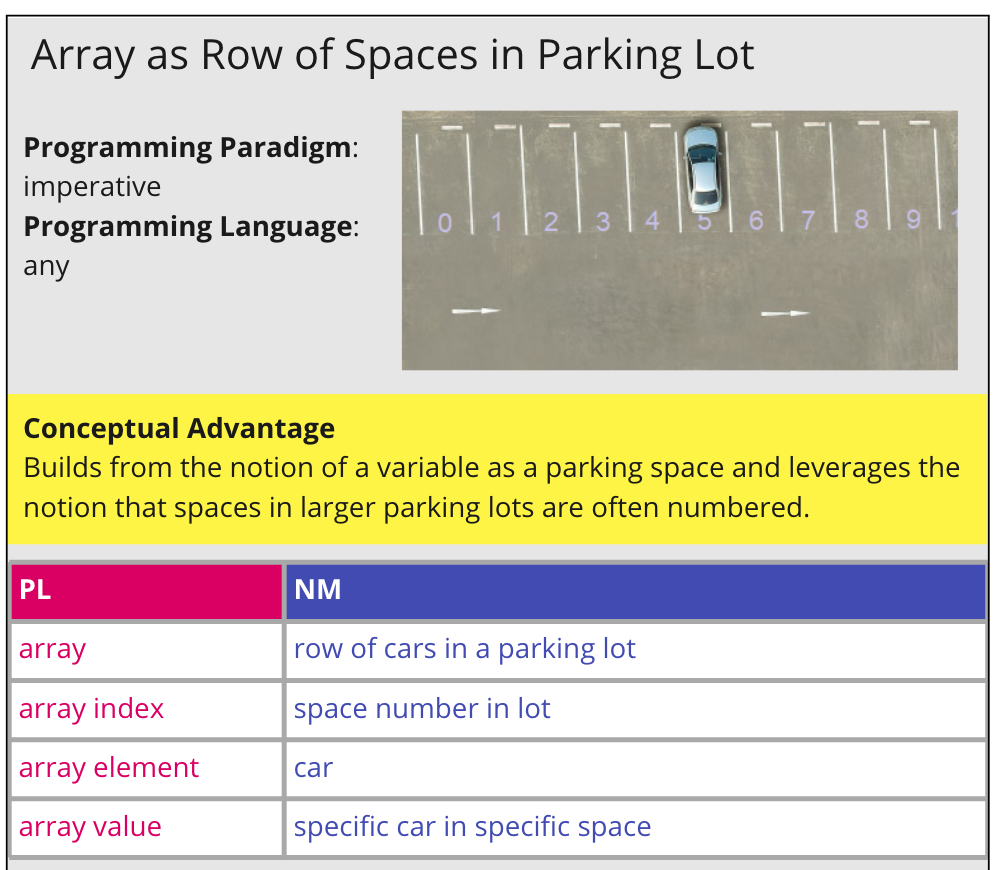
\includegraphics[width=.50\textwidth]{images/nm-definition-cards/nm-array-as-row-of-spaces-in-parking-lot-cut}
    \end{tabular}
     \caption{The ``Array as Row of Spaces in Parking Lot'' \nm{} captured by~\citet{fincherNotionalMachinesComputing2020}.}
    \label{fig:parkingSpaces}
% \end{figure}
\end{wrapfigure}

% - example: Array as Row of Parking Spaces
For example,
\citet{fincherNotionalMachinesComputing2020} describe the
``Array as Row of Spaces in Parking Lot'' \nm{}.
Figure~\ref{fig:parkingSpaces} shows part of their card summarizing it.
Notice the parallels between the programming language (PL) and the notional machine (NM).
% problem: empty parking space
Consider Java, a language commonly used in programming courses.
In Java,
when an array of objects is allocated,
all its slots contain
\mintinline{java}{null},
which means these slots don't contain a reference to any object.
This would be reasonably represented in the notional machine as an empty parking lot.
But if instead of an array of objects, we have an array of
\mintinline{java}{int}s,
for example,
then when we instantiate an array,
all its slots contain
\mintinline{java}{0},
which is not the absence of a number but a number like any other.
%
% other problems
A student could also reasonably question whether
one can park a car in a slot that is already occupied by another car,
or whether
one has to remove a car from a spot to park another car in the same spot.
%
In fact, the authors point out that,
``the effectiveness of the analogy depends on
%student knowledge of numbered parking spaces and
[...]
how well that models the semantics of the programming language.''


% - What properties should a NM satisfy?
\subsection{Soundness of \NMs{} via Simulation}
To avoid
these issues,
we need to make sure that a \nm{} 
is indeed an accurate abstraction.
%
Although
the more general view of
notional machines
as ``pedagogic devices to assist the understanding of some aspect of programs or programming''~\citep{fincherNotionalMachinesComputing2020}
makes no direct reference to programming languages,
programs are expressed in programming languages
% be it text based or not
so we will look at these ``aspects of programs''
through the lens of how they are realized by some programming language.
%
If a \nm{}
represents
a part of the operational semantics of a programming language,
for example,
then
this
representation
should be sound, in the sense that
steps in the \nm{}
correspond to steps in the operational semantics of the programming language.

%We say,
%informally,
%that
%a \nm{} is \emph{sound} if it is: 
%\begin{itemize}
%    \item a proper abstraction: it represents one or more aspects of the programming language and no superfluous aspects;
%    \item consistent with the corresponding programming language: steps in the \nm{} correspond to steps in the language semantics, and lead to similar results.
%\end{itemize}

Showing the soundness of a \nm{}
% with respect to some lang?
amounts to demonstrating that
the \nm{} \emph{simulates}
(in the sense described by~\citet{milnerAlgebraicDefinitionSimulation1971})
%the operational semantics of the underlying programming language
the aspect of programs under the focus of the \nm{}.
%This aspect under focus can be, for example, the operational semantics of a programming language.
% More precisely, the \nm{} simulates the operations of the semantics that it focuses on.
%
This property can be given in the form of a commutative diagram.
%We will present several such diagrams throughout this work.
%
Milner's simulation was also used
by~\citet{hoareProofCorrectnessData1972}
to establish a definition of
the correctness of
an `abstract' data type representation
with respect to
its corresponding `concrete' data type representation.
%
\citet{cousotAbstractInterpretationUnified1977} use a similar commutative diagram to simulate concrete computations in their abstract interpretation framework.
%
This interpretation of simulation
also captures the relationship between a \nm{} and the underlying programming language
because
% that's exactly what
a \nm{} is indeed an \emph{abstraction} of some aspect of interest.


\subsection{Contributions}
% - contributions
This paper makes the following contributions:
\begin{itemize}
    \item A formal definition of sound \nm{} based on simulation (Section~\ref{sec:soundnessDefinition}).
    \item A methodology for designing \nms{} that are sound by construction.

        It consists of
        deriving part of the notional machine
        by leveraging
        the relationship between
        the abstract representation of the notional machine
        and
        the abstract syntax of the programming language under its focus.

        We demonstrate the methodology by applying it
        to a combination of various
        small programming languages,
        \nms{},
        and
        aspects of programming language semantics
        (Section~\ref{chr:Modeling}).

    \item A methodology for analyzing \nms{} with respect to their soundness.

        It consists of
        modelling the notional machine and
        the aspect of the programming language under its focus,
        %
        relating them via simulation. %and
        %
        %using property-based testing to find counterexamples where the simulation fails.

        We
        demonstrate
        %evaluate
        the methodology by
        % applying it
        analyzing
        % \emph{M2} is applied to
        existing \nms{},
        sometimes
        pointing out unsoundnesses, and suggesting directions for improvement (Section~\ref{chr:RevealingInconsistencies}).
\end{itemize}

A brief discussion about the distinction between the abstract and concrete representations of a notional machine
follows
in Section~\ref{sec:ConcreteSyntax}.
We then
evaluate, in Section~\ref{chr:Evaluation}, the entire framework  %we are proposing to reason about notional machines
by comparing the notional machines that appeared
in Section~\ref{chr:Modeling} and Section~\ref{chr:RevealingInconsistencies}
to an existing dataset of \numOfNMs notional machines.
We classify the notional machines in the dataset according to various dimensions and show that the notional machines we analyzed are representative of the design space of notional machines used in practice.
Section~\ref{sec:RelatedWork} discusses related work
and Section~\ref{sec:Conclusions} concludes.




\section{Designing Sound Notional Machines}
\label{chr:Modeling}


We can only begin to talk about the soundness of a notional machine if we have a
formal description of the programming language the notional machine is focused
on.
%
We use a set of small programming languages with well-known formalizations
described in
Pierce's Types and Programming Languages (TAPL) book~\citep{pierceTypesProgrammingLanguages2002}.
The languages are used to
explore different aspects of programming language semantics.
%
%Throughout this chapter,
%these languages are used
%in various examples
%that explore different aspects of the design of notional machines.
%
Table~\ref{tab:examples-designing-nms}
shows
the notional machines
we use in this section
as well as
the corresponding programming language
and aspect of the semantics of the programming language
that the notional machine focuses on.
%
We use the first example also to introduce the definition of soundness for notional machines.

We model each programming language and notional machine in Haskell.
The models are executable,
so they include implementations of the programming languages
(including parsers, interpreters, and type-checkers),
the notional machines,
and the relationship between them%
\footnote{%
The artifact containing a superset of the examples in this paper
is at
\href{https://zenodo.org/doi/10.5281/zenodo.12609636}{10.5281/zenodo.12609636}.
%\url{https://github.com/LuCEresearchlab/sound-notional-machines}.
}.
The soundness proofs presented in this section are done using equational reasoning~\citep{gibbonsCalculatingFunctionalPrograms2002,birdAlgebraicIdentitiesProgram1989}.
%An implementation of the commutative diagrams of all the \nms{} presented in the thesis is available in an accompanying artifact.

\begin{table}[]
    \centering
    \begin{tabular}{|r||l|l|l|}
        \hline
        \textbf{Section}            & \textbf{Notional Machine}           & \textbf{Programming Language}    & \textbf{Focus}      \\ \hline\hline
        \ref{sec:ExpTree}  & \nmName{ExpTree}           & \plName{UntypedLambda}  & Evaluation \\ \hline
        \ref{sec:ExpTutor} & \nmName{ExpTutorDiagram}   & \plName{UntypedLambda}  & Evaluation \\ \hline
        % \ref{sec:Reduct} & \nmName{Reduct} & \plName{UntypedLambda} & step\\\hline
        % \ref{sec:AlligatorEggs} & \nmName{Alligator} & \plName{UntypedLambda} & step\\\hline
        \ref{sec:State}    & \nmName{TAPLMemoryDiagram} & \plName{TypedLambdaRef} & Evaluation (Refs) \\ \hline
        \ref{sec:Typing}   & \nmName{TypedExpTutorDiagram}   & \plName{TypedArith}     & Type-checking      \\ \hline
    \end{tabular}
    \caption{Notional machines, programming languages, and aspects of focus
    used in Section~\ref{chr:Modeling}.}
    \label{tab:examples-designing-nms}
\end{table}

\input{sections/BijectiveNM}

\input{sections/InjectiveNM}

\input{sections/TAPLMemoryDiagramNM}

\input{sections/TypedExpTutorNM}




%%%%%%%%%%%%%%%%%%%%%%%%%%%%%%%%%%%%%%
% \section{Conclusion}
% In this chapter, we have defined sound notional machines
% and shown how we can use the definition to devise a methodology to design notional machines that are sound by construction.
% We used the methodology to design
% different notional machines that
% focus on various aspects of
% multiple programming languages.
% In the next chapter, 
% we will use the definition to devise a methodology for analyzing existing notional machines.

\section{Analyzing Existing Notional Machines}
\label{chr:RevealingInconsistencies}

So far we have seen
how we can design sound \nms{} by
constructing \ensuremath{\Varid{f}_{\Conid{NM}}} using \ensuremath{\Varid{f}_{\Conid{PL}}} and
functions that convert between \ensuremath{\Conid{A}_{\Conid{PL}}} and \ensuremath{\Conid{A}_{\Conid{NM}}}.
%
Now we will analyze existing \nms{},
using their informal description to construct all components of the commutative diagram.
In particular, here,
we have a description
of \ensuremath{\Varid{f}_{\Conid{NM}}} entirely in terms of \ensuremath{\Conid{A}_{\Conid{NM}}}.
%
We then use property-based testing, using the soundness condition as a property,
to uncover unsoundnesses
and suggest improvements that eliminate them.
%
Table~\ref{tab:examples-fixing-nms}
shows
the notional machines
we use in this section
as well as
the corresponding programming language
and aspect of the semantics of the programming language
that the notional machine focuses on.

\begin{table}[]
    \centering
    \begin{tabular}{|r||l|l|l|}
        \hline
        \textbf{Section}            & \textbf{Notional Machine}           & \textbf{Programming Language}    & \textbf{Focus}      \\ \hline\hline
        \ref{sec:AlligatorEggs} & \nmName{Alligator} & \plName{UntypedLambda} & Evaluation \\ \hline
        \ref{sec:ListAsStack}  & \nmName{ListAsStack}           & -  & Data Structure (List) \\ \hline
        \ref{sec:ArrayAsParkingSpots} & \nmName{ArrayAsParkingSpots}   & \plName{Java}  & Evaluation (Arrays) \\ \hline
        % \ref{sec:Reduct} & \nmName{Reduct} & \plName{UntypedLambda} & step\\\hline
    \end{tabular}
    \caption{Notional machines, programming languages, and aspects of focus
    used in Section~\ref{chr:RevealingInconsistencies}.}
    \label{tab:examples-fixing-nms}
\end{table}


\input{sections/AlligatorNM}

\input{sections/ListAsStackNM}

\input{sections/ArrayAsParkingSpotsNM}






%%%%%%%%%%%%%%%%%%%%%%%%%%%%%%%%%%%%%%
%\section{Conclusion}

%In this chapter,
%we have seen
%how we can
%analyze existing notional machines
%with respect to their soundness
%and, as a result,
%find inconsistencies and improve them.
%%
%We also discussed the challenges of designing a concrete representation for a notional machine.

%The analyses in this chapter
%were made simpler by our use of \plName{UntypedLambda} as
%the programming language under the focus of the notional machines.
%%
%In contrast,
%in the next chapter,
%we will use essentially the same technique to analyze and improve a notional machine that is focused on Java,
%a much larger language.


\input{sections/ConcreteSyntax}
\section{Evaluation}
\label{chr:Evaluation}

%We then
%evaluate the entire framework
%by comparing the notional machines that appeared
%in Section~\ref{chr:Modeling} and Section~\ref{chr:RevealingInconsistencies}
%to an existing dataset of \numOfNMs notional machines.
%
%We classify the notional machines in the dataset according to various dimensions and show that the notional machines we analyzed are representative of the design space of notional machines used in practice.

The notional machines we presented not only exemplify how to use our framework to reason about notional machines
but also were chosen to be representative of the design space of notional machines used in practice.
%
To characterize this design space we analyzed the notional machines in the dataset collected by~\citet{fincherNotionalMachinesComputing2020}
and classified them according to three dimensions: form, focus, and language construct.
%
For each dimension,
we present the categories of the dimension
and for each category
we show
the number of notional machines in that category,
the percentage that number represents of the total,
and
the sections of the paper containing notional machines that fall into that category.
%
The notional machines are often not precesily described
so we often had to make assumptions about
their characteristics,
how they relate to an underlying programming language,
and how they are used to teach programming concepts.

\begin{wrapfigure}{r}{.53\textwidth}
%\begin{table}[]
\begin{tabular}{|l||r|r|l|}
\hline
\textbf{Form}  & \textbf{Num} & \textbf{Perc.} & \textbf{Covered} \\
\hline
\hline
Metaphorical  &  22  &  56.41\% & \ref{sec:ListAsStack} \ref{sec:ArrayAsParkingSpots} \ref{sec:AlligatorEggs} \\ \hline
Diagramatic  &  16  &  41.03\% & \ref{sec:ExpTree} \ref{sec:ExpTutor} \ref{sec:State} \ref{sec:Typing} \\ \hline
Both  &  1  &  2.56\% & - \\ \hline
\hline
\textbf{Total} & \numOfNMs    & 100.00\%   & -   \\
\hline
\end{tabular}
\captionof{table}{Notional machines in the dataset published by \citet{fincherNotionalMachinesComputing2020} classified according to their form.}
\label{tab:nm-classification-form}
%\end{table}
\end{wrapfigure}

%
The form (Table~\ref{tab:nm-classification-form}) of
a notional machine
can be
metaphorical (primarely inspired by and represented with real world objects) or
diagrammatic (represented with diagrams).
The distinction between the two is not always clear-cut,
given that
a notional machine may mix both forms
and
some real world objects can be represented diagrammatically.
%
Nevertheless, this distinction is useful because metaphorical notional machines may be more difficult to be made sound, given the existing degrees of freedom and constraints of the real world objects they are inspired by.


Most notional machines in the dataset focus (Table~\ref{tab:nm-classification-broad-focus})
on the runtime semantics (Evaluation) of a programming language construct
(or set of conceptually related constructs)
so
%
we further
break down these notional machines into the constructs they are primarely focused on (Table~\ref{tab:nm-classification-narrow-focus}).
%
Some entries in the table refer to sets of related constructs.
For example,
the category Control Flow encompasses constructs like loops and conditional statements, which primarily affect control flow.
%
%
%\nmName{TAPLMemoryDiagram} (Section~\ref{sec:State}),
%for example,
%represents the runtime semantics of all constructs of \plName{TypedLambdaRef}
%but would be classified as primarely focused on references.
%
Here the classification is also not clear-cut,
not only because a notional machine may focus on multiple constructs
but also because some constructs are related to others.
For example,
notional machines that focus on functions often (although not always) represent variables as well
but only the ones that solely (or primarily) focus on variables are classified as such.
%
The category Misc
includes five notional machines each of which focuses on a different construct:
String literal,
Procedure (side-effecting functions),
Objects,
Instructions (lower level operations),
and
one that is not clear from the description.

%todo evaluation is a leap of faith...

\begin{table}[h]
    \centering
    \begin{minipage}{0.48\textwidth}
        \centering
        \begin{tabular}{|l||r|r|p{1.4cm}|}
\hline
\textbf{Focus} & \textbf{Num} & \textbf{Perc.} & \textbf{Covered} \\
\hline
\hline
Evaluation  &  32  &  82.05\% & \ref{sec:ExpTree} \ref{sec:ExpTutor} \ref{sec:State} \ref{sec:ArrayAsParkingSpots} \ref{sec:AlligatorEggs} \\ \hline
Type-checking  &  2  &  5.13\% &  \ref{sec:Typing} \\ \hline
Parsing  &  2  &  5.13\% & no \\ \hline
Data Structure  &  2  &  5.13\% &  \ref{sec:ListAsStack} \\ \hline
Logic Gates  &  1  &  2.56\% & no \\ \hline
\hline
\textbf{Total} & \numOfNMs    & 100.00\%  & -   \\
\hline
\end{tabular}
\caption{Notional machines in the dataset published by \citet{fincherNotionalMachinesComputing2020} classified according to their focus.}
\label{tab:nm-classification-broad-focus}
    \end{minipage}\hfill
    \begin{minipage}{0.48\textwidth}
        \centering
\begin{tabular}{|l||r|r|l|}
\hline
\textbf{Construct} & \textbf{Num} & \textbf{Perc.} & \textbf{Covered} \\
\hline
\hline
References  &  8  &  20.51\% & \ref{sec:State} \\ \hline
Functions  &  5  &  12.82\% & \ref{sec:ExpTree} \ref{sec:ExpTutor} \\ \hline
Variables  &  4  &  10.26\% & \ref{sec:ExpTree} \ref{sec:ExpTutor} \ref{sec:State} \\ \hline
Arrays  &  4  &  10.26\% & \ref{sec:ArrayAsParkingSpots} \\ \hline
Methods  &  3  &  7.69\% & no \\ \hline
Control Flow  &  2  &  5.13\% & no \\ \hline
Expressions  &  1  &  2.56\% & \ref{sec:ExpTree} \ref{sec:ExpTutor} \\ \hline
\hline
Misc  &  5  &  12.82\% & no \\ \hline
%Memory          & 7     & 18.92\%   & yes \\ \hline
%Variables       & 5     & 13.51\%   & yes \\ \hline
%Arrays          & 4     & 10.81\%   & yes \\ \hline
%Functions       & 3     & 8.11\%    & yes \\ \hline
%Expression      & 3     & 8.11\%    & yes \\ \hline
%Method Calls    & 2     & 5.41\%    & no  \\ \hline
%Control Flow    & 2     & 5.41\%    & no  \\ \hline
%Call Stack      & 2     & 5.41\%    & no  \\ \hline
%??              & 2     & 5.41\%    & -   \\ \hline
%Tracing         & 1     & 2.70\%    & no  \\ \hline
%Recursion       & 1     & 2.70\%    & yes \\ \hline
%Parsing         & 1     & 2.70\%    & yes \\ \hline
%Objects         & 1     & 2.70\%    & no  \\ \hline
%Logic Operation & 1     & 2.70\%    & no  \\ \hline
%List            & 1     & 2.70\%    & yes \\ \hline
%HashSets        & 1     & 2.70\%    & no  \\ \hline
\hline
\textbf{Total} & 32    & 82.05\%   & -   \\
\hline
\end{tabular}
\caption{Notional machines that focus on evaluation broken down by the set of construct they focus on.}
\label{tab:nm-classification-narrow-focus}
    \end{minipage}
\end{table}





%todo: cut values 1 and 2 and explain in text

%We then classified the notion of machines shown in Section~\ref{chr:Modeling} and Section~\ref{chr:RevealingInconsistencies} according to these dimensions.
%
%\begin{table}[]
%\begin{tabular}{|l||l|l|l|}
%\hline
%\textbf{Notional Machine}      & \textbf{Form} & \textbf{Broad Focus} & \textbf{Focused Construct} \\ \hline
%\hline
%\hline
%Array a Row of Parkings Spaces & Analogy        & Evaluation     & Arrays       \\ \hline
%List a Stack of Boxes          & Analogy        & Data Structure & List         \\ \hline
%ExpTree                        & Representation & Evaluation     & -            \\ \hline
%ExpTutorDiagram                & Representation & Evaluation     & -            \\ \hline
%TAPLMemoryDiagram              & Representation & Evaluation     & References   \\ \hline
%TypedExpTutorDiagram           & Representation & Type-checking  & -            \\ \hline
%AlligatorEggs                  & Analogy        & Evaluation     & -            \\ \hline
%\end{tabular}
%\caption{Notional machines analyzed in this paper classified according to dare form, broad focus, and narrow focus.}
%\label{tab:our-nm-classification}
%\end{table}

\subsection{Expressing Complex Language Semantics}
\label{sec:more-complexity}

% - modeling layers
Although
the notional machines presented here as well as in the dataset by \citet{fincherNotionalMachinesComputing2020}
focus on aspects of program semantics that one may consider simple,
the framework we presented can be used to reason about more complex aspects of program semantics.
%
An example
is
the conceptual models
to reason about Ownership Types in Rust by~\citet{crichtonGroundedConceptualModel2023}.
% fits nicely in our framework
The authors present two models: a dynamic and a static one.
In our framework,
each model can be seen as a notional machine.
The authors divide each model into a formal model (about which formal statements can be made), which would correspond to the abstract representation of the notional machine,
and an informal model, which would correspond to the concrete representation of the notional machine.
%
In the dynamic model,
our PL layer would be the Rust language
and
our NM layer would be Miri.
%
In the static model,
our PL layer would be the Polonius model of borrow checking
and
our NM layer would be the \emph{permissions model} of borrow checking
(introduced by the authors).



% ### Notional Machines vs. Conceptual Model
% 
% The original acception (or acceptation) of notional machine referred to dynamic semantics but the Working Group showed that the modern acception of the term is broader. The definition as “pedagogical devices that assist the understanding of some aspect of programs are programming” is more aligned with modern uses of the term so include also static semantics. For example, x/50 notional machines described in the paper are about static semantic. In this way, notional machine is equal to conceptual model ( the working group also had something to about this).
% 
% An advantage of using the term conceptual model is that it seems it’s connotation is of something that is less ad-hoc. Notional machine seems something more like a toy to help teaching so something less foundational. An interesting use of the term conceptual model in the paper is in the phrase “to help learners acquire a conceptual model valid for common task”. So a conceptual model is something you can acquire, something on the same level of  “model of computation”. But that’s what we mean when we use the term notional machine: a didactic model of computation or a didactic model to reason about computation. It’s interesting to look at a few examples to elicit the differences in use of these terms. For example, a Stack&Heap diagram is in the same level of the Environment Model which is on the same level of the Substitution Model. All of these are models of computation, are models used to reason about computation. But although one would say that the S&H diagram is a notional machine, few would say the substitution model is a notional machine.
% 
% Another connotation of conceptual is “way of thinking”, e.g. about semantics. That’s good because NM seems optional and costly and conceptual model is required!



% From: A Grounded Conceptual Model for Ownership Types in Rust
% Our work continues a line of CS education research about conceptual models. Bayman and Mayer [1988] ￿rst showed that an appropriate conceptual model for BASIC could help students “develop fewer misconceptions [...] and perform better on transfer tests.” du Boulay [1986] coined the term “notional machine” for conceptual models speci￿cally of a language’s dynamic semantics, which has received renewed focus in recent years [Dickson et al. 2020]. Our work di￿ers from most research on notional machines by focusing equally on a conceptual model of static semantics.
% 
% Layers:
% Informal model <--> concrete representation
% Formal model   <--> abstract representation
% Implementation


% From: Notional Machines in Computing Education: The Education of Attention
% “A notional machine is the idealised model of the computer implied by the constructs of the programming language.”
% NM is effectively a special kind of conceptual model.

%%%%%%%%%%%%%%%%%%%%%%%%%%%%%%%%%%%%%%
\section{Related Work}
\label{sec:RelatedWork}


% - nms are for static and dynamic semantics
The term notional machine
was coined by~\citet{duboulayDifficultiesLearningProgram1986} to refer to
``the idealised model of the computer implied by the constructs of the programming language''.
Therefore it
restricts the use of notional machines as means to help understand the runtime behavior of a program or the dynamic semantics of a language.
\citet{fincherNotionalMachinesComputing2020}, a working group that included du Boulay,
has a thorough literature review and discussion of the term notional machine
and
established a broader definition
as
``pedagogic devices to assist the understanding of some aspect of programs or programming'',
which includes
uses of notional machines as means to help understand the static semantics of a language.
% e.g.
The ``Expressions as Trees'' notional machine~\citep{fincherNotionalMachinesComputing2020},
for example,
is used for both.
We adopt here this broader view of notional machine.

% - nms vs. conceptual models
Another related and important term is conceptual model.
\citet{fincherNotionalMachinesComputing2020} states that a
``notional machine is effectively a special kind of conceptual model.''
That's important because
conceptual models,
such as the Substitution Model and the Environment Model used
in the SICP book (Structure and Interpretation of Computer Programs)~\cite{abelsonStructureInterpretationComputer1996},
and SICPJS~\cite{abelsonStructureInterpretationComputer2022},
for example,
are well understood to be essential for reasoning about programs.
Notional machines that are sound are indeed conceptual models.
The concrete representation of the notional machine
can be thought of as embodying the visualization of this conceptual model.

%\begin{meta}
%\begin{itemize}
%    \item Felleisen ``On the expressive power of programming languages''~\cite{felleisenExpressivePowerProgramming1991}
%\end{itemize}
%\end{meta}
The idea of simulating or representing a program by means of another program is an old one, 
and was first studied in detail in the 1970s by~\citet{milnerAlgebraicDefinitionSimulation1971} and~\citet{hoareProofCorrectnessData1972}. 
Many of our \nms{} illustrate a reduction, stepping, or evaluation `aspect' of a programming language. 
\citet{wadlerProgrammingLanguageFoundations2020} descriptions of how to relate such reduction systems with simulation, lock-step simulation, and bisimulation.
The commutative diagram describing the desired property of a \nm{} appears in many places in the literature, and is a basic concept in Category Theory. Closer to our application is its use as `promotion condition'~\cite{birdPromotionAccumulationStrategies1984,wangRefactoringPatternMatching2013}.
%Some notional machines focus on representing reduction,
%and thus $f$ represent reduction rules.
%For other notional machines,
%the $f$ do not represent reduction rules,
%but they may be arbitrary projections to some property.

% Berry and K\"olling~\cite{berryDesignImplementationNotional2013}
Where computing education researchers capture program behavior through \nms{}, programming language researchers instead use semantics~\cite{krishnamurthiProgrammingParadigms2019}. Our work can be seen as a rather standard approach to show the correctness of one kind of semantics of (part of) a programming language, most often the operational semantics, with respect to another semantics, often a reduction semantics. An example of such an approach has been described by~\citet{clementsModelingAlgebraicStepper2001}, whose Elaboration Theorem describes a property that is very similar to our soundness requirement.
%
The lack of a formal approach to showing the soundness of \nms{} is also noted by~\citet{pollockTheiaAutomaticallyGenerating2019}, who develop a formal approach to specifying correct program state visualization tools, based on an executable semantics of the programming language formulated in the K framework~\citep{rosuOverviewSemanticFramework2010}.
In this paper we study a broader collection of \nms{} than just program state visualization tools, and we apply our approach to study the soundness of \nms{}.



Computing educators practitioners use a diverse set of \nms{}~\cite{fincherNotionalMachinesComputing2020}.
%Dickson and Dragon~\cite{dicksonMemoryDiagramAll2021} describe an approach to consistently developing memory diagrams, but they do not formalise their approach. 
%Dickson et al.~\cite{dicksonExperiencesImplementingUtilizing2022} ...
Some \nms{} form the basis of automated tools.
The BlueJ IDE,
which features prominently in an introductory programming textbook~\cite{kollingObjectsFirstJava2017},
includes a graphical user interface to visualize objects, invoke methods, and inspect object state.
PythonTutor~\cite{guoOnlinePythonTutor2013}, an embeddable web-based program visualization system,
is used by hundreds of thousands of users to visualize the execution of code written in Python, Java, JavaScript, and other programming languages.
UUhistle~\cite{sorvaUUhistleSoftwareTool2010}, a ``visual program simulation'' system, takes a different approach:
instead of visualizing program executions, it requires students to perform the execution steps in a constrained interactive environment.
When developing such widely used tools, starting from a sound \nm{} is essential.


\citet{dicksonExperiencesImplementingUtilizing2022} discuss the issues around developing and using a \nm{} in class. They note, amongst others, ``that a \nm{} must by definition be correct, but a student's mental model of the \nm{} often is not'', and that ``specifying a \nm{} was more difficult than we thought it would be''. Our work can help in developing a \nm{}, and pointing out flaws in it. 



%%%%%%%%%%%%%%%%%%%%%%%%%%%%%%%%%%%%%%
\section{Conclusions}
\label{sec:Conclusions}

% - problem
Notional machines
%is a pedagogic device to assist the understanding of some aspect of programs or programming
%under focus by the notional machine.
%%they are popular
%They
are popular in computer science education,
commonly used both by instructors in their teaching practice
as well as by researchers.
%
Despite
their popularity,
there has been no precise formal characterization of
what should be the relationship between
a notional machine
and
the aspect
of the programming language
under its focus
%
that would allow one to
evaluate whether or not they are consistent with each other.
%
%
% - solution
% -- definition
We, therefore, introduced
a definition
of soundness for notional machines.
The definition is based on
%the idea of
simulation,
a
well-established notion
widely used in many areas of computer science.
%to proofs of correctness of data representations.
%
Demonstrating soundness essentially
amounts to
constructing
a commutative diagram relating the \nm{}
with the object of its focus.


% -- methodologies
Using this definition,
we
showed how we can
(1)
systematically
design notional machines that are sound by construction,
%
%which
%we demonstrate
%with a series of examples
%that explore different
%notional machines
%and
%aspects of programming language semantics,
and
(2)
analyze existing notional machines
to uncover inconsistencies
and suggest improvements.


% -- abstract versus concrete
An important insight
in the process
is to
distinguish between
the concrete representation of the notional machine
(typically visual)
and its abstract representation,
about which we can make formal statements.
%
This distinction is akin to the distinction between
the concrete and the abstract syntaxes of a programming language.
 
% -- evaluation
We then evaluated 
how applicable our approach is
to notional machines
actually used in practice.
%
%We classify the notional machines in the dataset according to various dimensions
Using
a set of
previously published notional machines
used in practice,
we characterize their design space
%
and show that
the notional machines we analyzed using our approach
are representative of that design space.


% - takeaways
% -- reasoning about notional machines
This work intends more generally to establish a
%The approach presented here is meant more broadly as a general
framework to reason about notional machines,
placing the research on notional machines on firmer ground.
As such,
it can be
used
to address challenges
such as the design, analysis, and evaluation of notional machines,
and
the construction of automated tools based on notional machines.




%%
%% The acknowledgments section is defined using the "acks" environment
%% (and NOT an unnumbered section). This ensures the proper
%% identification of the section in the article metadata, and the
%% consistent spelling of the heading.
\begin{acks}
acknowledgments
\end{acks}

%%
%% The next two lines define the bibliography style to be used, and
%% the bibliography file.
\bibliographystyle{ACM-Reference-Format}
\bibliography{biblio}

\newpage

%%
%% If your work has an appendix, this is the place to put it.
\appendix

\section{Programming Language Definitions}
\label{chr:appendix-programming-language-definitions}

% The languages used in Chapters~\ref{chr:Modeling} and~\ref{chr:RevealingInconsistencies}
% are defined in this appendix
% using operational semantics.
The programming languages used throughout the paper
mostly follows
the presentation in
the book
Types and Programming Languages by~\citet{pierceTypesProgrammingLanguages2002}
with minor changes.
In particular,
italics are used for metavariables and
the axioms
in the reduction (evaluation) rules and
typing rules
are shown with explicitly empty premises.


\subsection{UntypedLambda}
\label{sec:language-definition-untypedlambda}

Figure~\ref{fig:language-definition-untypedlambda}
shows the syntax and evaluation rules
for the untyped lambda calculus by~\citet{churchUnsolvableProblemElementary1936a,churchCalculiLambdaconversion1941},
that we have referred to as \plName{UntypedLambda}.
%
This language is used in
Sections~\ref{sec:ExpTree},
\ref{sec:ExpTutor},
%\ref{sec:Reduct},
and~\ref{sec:AlligatorEggs}
.
%
% The book contains a good explanation
% of the pitfalls of the substitution operation
% in the Rule~\textsc{E-AppAbs},
% which was the source of the problem
% found in \nmName{Alligator}~(Section~\ref{sec:AlligatorEggs}).


\begin{figure}[h]
\footnotesize
\begin{tabular}{p{0.47\textwidth}|p{0.47\textwidth}}
    \textbf{Syntax} & \textbf{Evaluation} \tabularnewline[1em]
    \begin{tabular}{r@{\hspace{0.5em}}r@{\hspace{0.5em}}lr}
        $t$ & ::= &              & terms:      \\
            &     & $x$          & variable    \\
            & |   & $\abs{x}{t}$ & abstraction \\
            & |   & $\app{t}{t}$ & application \\
            &     &              &             \\
        $v$ & ::= &              & values:     \\
            &     & $\abs{x}{t}$ &
    \end{tabular}
&
    \renewcommand{\arraystretch}{3.0}
    \begin{tabular}{cr}
        $\inferrule*[Right=E-AppAbs]
            { }
            {\app{(\abs{x}{t_{12}})}{v_2}\ \longrightarrow\ \subst{v_2}{x}{t_{12}}}$ \label{rule:E-AppAbs} & \\
        $\inferrule*[Right=E-App1]
            {t_1\ \longrightarrow\ t_1'}
            {\app{t_1}{t_2}\ \longrightarrow\ \app{t_1'}{t_2}}$ & \\
        $\inferrule*[Right=E-App2]
            {t_2\ \longrightarrow\ t_2'}
            {\app{v_1}{t_2}\ \longrightarrow\ \app{v_1}{t_2'}}$ & 
    \end{tabular}
\end{tabular}
\caption{The untyped lambda calculus (\plName{UntypedLambda}).}
\label{fig:language-definition-untypedlambda}
\end{figure}
  

\subsection{TypedArith}
\label{sec:language-definition-typedarith}

We define here the language \plName{TypedArith},
used in Section~\ref{sec:Typing}.
Figure~\ref{fig:language-definition-typedarith}
shows its syntax and evaluation (reduction) rules
and Figure~\ref{fig:language-definition-typedarith-types}
shows its typing rules.
%but here all the rules are shown together.
%
The appeal
of using this language to present a notional machine
focused on the types is its simplicity.
Terms don't require type annotations
and the typing rules don't require a type environment.
In fact,
Pierce uses it as
the simplest example of a typed language
when introducing type safety.



\begin{figure}[h]
\footnotesize
\begin{tabular}{p{0.47\textwidth}|p{0.47\textwidth}}
    \textbf{Syntax} & \textbf{Evaluation} \tabularnewline[1em]
    \begin{tabular}{r@{\hspace{0.5em}}r@{\hspace{0.5em}}l@{\hspace{0.5em}}r}

              $t$ & ::= &                       & terms:          \\
                  &     & $\true$               & constant true   \\
                  & |   & $\false$              & constant false  \\
                  & |   & $\ift{t}{t}{t}$       & conditional     \\
                  & |   & $\zero$               & constant zero   \\
                  & |   & $\succt{t}$           & successor       \\
                  & |   & $\predt{t}$           & predecessor     \\
                  & |   & $\iszerot{t}$         & zero test       \\
                  &     &                       &                 \\
              $v$ & ::= &                       & values:         \\
                  &     & $\true$               &                 \\
                  & |   & $\false$              &                 \\
                  & |   & $\mathit{nv}$         &                 \\
                  &     &                       &                 \\
    $\mathit{nv}$ & ::= &                       & numeric values: \\
                  &     & $\zero$               &                 \\
                  & |   & $\succt{\mathit{nv}}$ &                 \\
    \end{tabular}
&
    \renewcommand{\arraystretch}{2.5}
    \begin{tabular}{c@{\hspace{0.5em}}r}
        $\inferrule*[Right=E-IfTrue]
            { }
            {\ift{\true}{t_2}{t_3}\ \longrightarrow\ t_2}$ & \\
        $\inferrule*[Right=E-IfFalse]
            { }
            {\ift{\false}{t_2}{t_3}\ \longrightarrow\ t_3}$ & \\
        $\inferrule*[Right=E-If]
            {t_1\ \longrightarrow\ t_1'}
            {\ift{t_1}{t_2}{t_3}\\\ \longrightarrow\ \ift{t_1'}{t_2}{t_3}}$ & \\
                        \vspace*{-1.5em} & \\[0.0em]
        $\inferrule*[Right=E-Succ]
            {t_1\ \longrightarrow\ t_1'}
            {\succt{t_1}\ \longrightarrow\ \succt{t_1'}}$ & \\
                        \vspace*{-1.5em} & \\[0.0em]
        $\inferrule*[Right=E-PredZero]
            { }
            {\predt{\zero}\ \longrightarrow\ \zero}$ & \\
        $\inferrule*[Right=E-PredSucc]
            { }
            {\predt{(\succt{\mathit{nv}_1})}\ \longrightarrow\ \mathit{nv}_1}$ & \\
        $\inferrule*[Right=E-Pred]
            {t_1\ \longrightarrow\ t_1'}
            {\predt{t_1}\ \longrightarrow\ \predt{t_1'}}$ & \\
                        \vspace*{-1.5em} & \\[0.0em]
        $\inferrule*[Right=E-IszeroZero]
            { }
            {\iszerot{\zero}\ \longrightarrow\ \true}$ & \\
        $\inferrule*[Right=E-IszeroSucc]
            { }
            {\iszerot{(\succt{\mathit{nv}_1})}\ \longrightarrow\ \false}$ & \\
        $\inferrule*[Right=E-IsZero]
            {t_1\ \longrightarrow\ t_1'}
            {\iszerot{t_1}\ \longrightarrow\ \iszerot{t_1'}}$ & 
    \end{tabular}
\end{tabular}
\caption{Syntax and reduction rules of the \plName{TypedArith} language.}
\label{fig:language-definition-typedarith}
\end{figure}


\begin{figure}[h]
\footnotesize
\begin{tabular}{p{0.47\textwidth}|p{0.47\textwidth}}
    \textbf{Syntax} & \textbf{Typing rules} \tabularnewline[1em]
    \begin{tabular}{r@{\hspace{0.5em}}r@{\hspace{0.5em}}l@{\hspace{1.0em}}r}
        $T$ & ::= &         & types:                  \\
            &     & $\Bool$ & type of booleans        \\
            & |   & $\Nat$  & type of natural numbers \\
    \end{tabular}
&
    \renewcommand{\arraystretch}{2.5}
    \begin{tabular}{cr}
        $\inferrule*[Right=T-True]
            { }
            {\true : \Bool}$ & \\
        $\inferrule*[Right=T-False]
            { }
            {\false : \Bool}$ & \\
        $\inferrule*[Right=T-If]
            {t_1 : \Bool \\ t_2 : T \\ t_3 : T}
            {\ift{t_1}{t_2}{t_3} : T}$ & \\
        $\inferrule*[Right=T-Zero]
            { }
            {\zero : \Nat}$ & \\
        $\inferrule*[Right=T-Succ]
            {t_1 : \Nat}
            {\succt{t_1} : \Nat}$ & \\
        $\inferrule*[Right=T-Pred]
            {t_1 : \Nat}
            {\predt{t_1} : \Nat}$ & \\
        $\inferrule*[Right=T-IsZero]
            {t_1 : \Nat}
            {\iszerot{t_1} : \Bool}$ & 
    \end{tabular}
\end{tabular}
\caption{Syntax of types and typing rules of the \plName{TypedArith} language.}
\label{fig:language-definition-typedarith-types}
\end{figure}



\subsection{TypedLambdaRef}
\label{sec:language-definition-typedlambdaref}

% \begin{meta}
% \begin{itemize}
%     \item Made of lambda simply typed lem the calculus plus type doris plus you init sequence references and tuples
%     \item Typing rules are missing because in the notion of machine we are focused on evaluation
%     \item  briefly explains superscript
%     \item  notice that the store which is manipulated in rules so and so needs to be carried over through all the other rules
%     \item Only the reduction rules for sequence references and to pose are shown. The reduction rules for the rest of the language are similar to what was shown before except for the store then needs to be thread through
% \end{itemize}
% \end{meta}

In Section~\ref{sec:State},
we showed the language \plName{TypedLambdaRef},
used
to design a notional machine that focuses on references.
%     \item Made of lambda simply typed lem the calculus plus type doris plus you init sequence references and tuples
This language is composed of
the simply-typed lambda calculus,
the \plName{TypedArith} language,
tuples,
the $\Unit$ type,
sequencing, and
references.
%
Our goal is again simplicity and
this is the simplest language we need for the examples in the book that use the diagram.
%
Figure~\ref{fig:language-definition-typedlambdaref} shows its syntax and evaluation (reduction) rules.
%     \item Only the reduction rules for sequence references and to pose are shown. The reduction rules for the rest of the language are similar to what was shown before except for the store then needs to be thread through
We show only
the reduction rules for
sequencing,
references, and
tuples
because
the rules for the rest of the language
are similar to what we showed before,
except for the store then needs to be threaded through all the rules.
%
Although that is a typed language,
we don't present its typing rules
because
the notional machine in Section~\ref{sec:State} is
focused only on its runtime behavior and not its types.


\begin{figure}[h]
\footnotesize
\begin{tabular}{p{0.47\textwidth}|p{0.47\textwidth}}
    \textbf{Syntax} & \textbf{Evaluation} \\[1em]
    \begin{tabular}{r@{\hspace{0.5em}}r@{\hspace{0.5em}}l@{\hspace{0.5em}}r}
        $t$ & ::= &                             & terms:              \\
            &     &                             &                     \\
            &     & $x$                         & variable            \\
            & |   & $\tyabs{x}{T}{t}$           & abstraction         \\
            & |   & $\app{t}{t}$                & application         \\
            &     &                             &                     \\
            & |   & $\true$                     & boolean true        \\
            & |   & $\false$                    & boolean false       \\
            & |   & $\zero$                     & zero                \\
            & |   & $\succt{t}$                 & successor           \\
            & |   & $\predt{t}$                 & predecessor         \\
            & |   & $\iszerot{t}$               & zero test           \\
            &     &                             &                     \\
            & |   & $\unit$                     & unit constant       \\
            & |   & $\seq{t}{t}$                & sequence            \\
            & |   & $\refr{t}$                  & reference creation  \\
            & |   & $\deref{t}$                 & dereference         \\
            & |   & $\assign{t}{t}$             & assignment          \\
            & |   & $l$                         & location            \\
            &     &                             &                     \\
            & |   & $\Tuple{{t_i}^{i\in 1..n}}$ & tuple               \\
            & |   & $\proj{t}{i}$               & projection          \\
            &     &                             &                     \\
        $v$ & ::= &                             & values:             \\
            &     & $\tyabs{x}{T}{t}$           &                     \\
            & |   & $\true$                     &                     \\
            & |   & $\false$                    &                     \\
            & |   & $\zero$                     &                     \\
            & |   & $\succt{v}$                 &                     \\
            & |   & $\unit$                     &                     \\
            & |   & $l$                         &                     \\
            & |   & $\Tuple{{v_i}^{i\in 1..n}}$ &                     \\
            &     &                             &                     \\
        $T$ & ::= &                             & types:              \\
            &     & $\Fun{T}{T}$                & function type       \\
            & |   & $\Bool$                     & boolean type        \\
            & |   & $\Nat$                      & natural number type \\
            & |   & $\Unit$                     & unit type           \\
            & |   & $\Ref{T}$                   & reference type      \\
            & |   & $\Tuple{{T_i}^{i\in 1..n}}$ & tuple type          \\
            &     &                             &                     \\
      $\mu$ & ::= &                             & store:              \\
            &     & $\emptyset$                 & empty store         \\
            & |   & $\mu, l \mapsto v$          & location binding    \\
    \end{tabular}
    &
    \renewcommand{\arraystretch}{2.5}
    \begin{tabular}{cr}
        $\inferrule*[Right=E-Seq] 
            {t_1 | \mu\ \longrightarrow\ t'_1 | \mu'}
            {\seq{t_1}{t_2} | \mu\ \longrightarrow\ \seq{t'_1}{t_2} | \mu'}$ & \\
        $\inferrule*[Right=E-SeqNext] 
            { }
            {\seq{\unit}{t_2} | \mu\ \longrightarrow\ t_2 | \mu}$ & \\
         & \\
        $\inferrule*[Right=E-RefV] 
            {l \notin \mathit{dom}(\mu)}
            {\refr{v_1} | \mu\ \longrightarrow\ l | (\mu, l \mapsto v_1)}$ & \\
        $\inferrule*[Right=E-Ref] 
            {t_1 | \mu\ \longrightarrow\ t'_1 | \mu'}
            {\refr{t_1} | \mu\ \longrightarrow\ \refr{t'_1} | \mu'}$ & \\
        $\inferrule*[Right=E-DerefLoc] 
            {\mu(l) = v}
            {\deref{l} | \mu\ \longrightarrow\ v | \mu}$ & \\
        $\inferrule*[Right=E-Deref] 
            {t_1 | \mu\ \longrightarrow\ t'_1 | \mu'}
            {\deref{t_1} | \mu\ \longrightarrow\ \deref{t'_1} | \mu'}$ & \\
        $\inferrule*[Right=E-Assign] 
            { }
            {\assign{l}{v_2} | \mu\ \longrightarrow\ \unit | [l \mapsto v_2]\mu}$ & \\
        $\inferrule*[Right=E-Assign1] 
            {t_1 | \mu\ \longrightarrow\ t'_1 | \mu'}
            {\assign{t_1}{t_2} | \mu\ \longrightarrow\ \assign{t'_1}{t_2} | \mu'}$ & \\
        $\inferrule*[Right=E-Assign2] 
            {t_2 | \mu\ \longrightarrow\ t'_2 | \mu'}
            {\assign{v_1}{t_2} | \mu\ \longrightarrow\ \assign{v_1}{t'_2} | \mu'}$ & \\
         & \\
        $\inferrule*[Right=E-ProjTuple] 
            { }
            {\proj{\Tuple{{v_i}^{i\in 1..n}}}{j} | \mu\ \longrightarrow\ v_j | \mu}$ & \\
        $\inferrule*[Right=E-Proj] 
            {t_1 | \mu\ \longrightarrow\ t'_1 | \mu'}
            {\proj{t_1}{i} | \mu\ \longrightarrow\ \proj{t'_1}{i} | \mu'}$ & \\
        $\inferrule*[Right=E-Tuple] 
            {t_j | \mu\ \longrightarrow\ t'_j | \mu'}
            {\Tuple{{v_i}^{i\in 1..j-1}, t_j, {t_k}^{k\in j+1..n}} | \mu \\
               \ \longrightarrow\ \Tuple{{v_i}^{i\in 1..j-1}, t'_j, {t_k}^{k\in j+1..n}} | \mu'}$ & \\
    \end{tabular}
\end{tabular}
\caption{\plName{TypedLambdaRef}: Syntax and Evaluation}
\label{fig:language-definition-typedlambdaref}
\end{figure}







\end{document}
\endinput
%%
%% End of file `sample-sigplan.tex'.
